\chapter{Score-Level Fusion}
\label{chap:score_fusion}
\section{Experimental Results}
To push the classification performance to its theoretical limit, we implemented Score-Level Fusion. Rather than relying on a single classification geometry, we fused the raw output scores of our two most complementary, high-performing models: the RBF Kernel SVM and the Tied GMM. We trained a prior-weighted Logistic Regression calibration model on these stacked score vectors to compute the optimal fusion weights and project them into a single, calibrated Log-Likelihood Ratio.
Table \ref{tab:fusion_eval_results} compares the Minimum and Actual DCF of the fused system against the performance of the individual calibrated models evaluated on the unseen Evaluation Set.
\begin{table}[H]
\centering
\caption{Score-Level Fusion Performance vs. Individual Calibrated Models (Evaluation Set).}
\label{tab:fusion_eval_results}
\resizebox{0.8\textwidth}{!}{
\begin{tabular}{llcc}
\toprule
\textbf{Model} & \textbf{Application Prior ($\tilde{\pi}$)} & \textbf{minDCF} & \textbf{actDCF} \\
\midrule
\multirow{3}{*}{\textbf{Calibrated SVM}}
& 0.1 & 0.459 & 0.495 \\
& 0.5 & 0.188 & 0.191 \\
& 0.9 & 0.432 & 0.437 \\
\midrule
\multirow{3}{*}{\textbf{Calibrated Tied GMM}}
& 0.1 & 0.407 & 0.448 \\
& 0.5 & 0.166 & 0.169 \\
& 0.9 & 0.365 & 0.371 \\
\midrule
\multirow{3}{*}{\textbf{Fused SVM + GMM}}
& 0.1 & \textbf{0.406} & \textbf{0.450} \\
& 0.5 & \textbf{0.166} & \textbf{0.168} \\
& 0.9 & \textbf{0.363} & \textbf{0.368} \\
\bottomrule
\end{tabular}
}
\end{table}
To analyze the continuous performance across all target applications, the Bayes Error plots comparing the Fused System against the individual SVM and GMM models are provided in Figures \ref{fig:fusion_vs_svm} and \ref{fig:fusion_vs_gmm}.
\begin{figure}[H]
\centering
\begin{minipage}{0.48\textwidth}
\centering
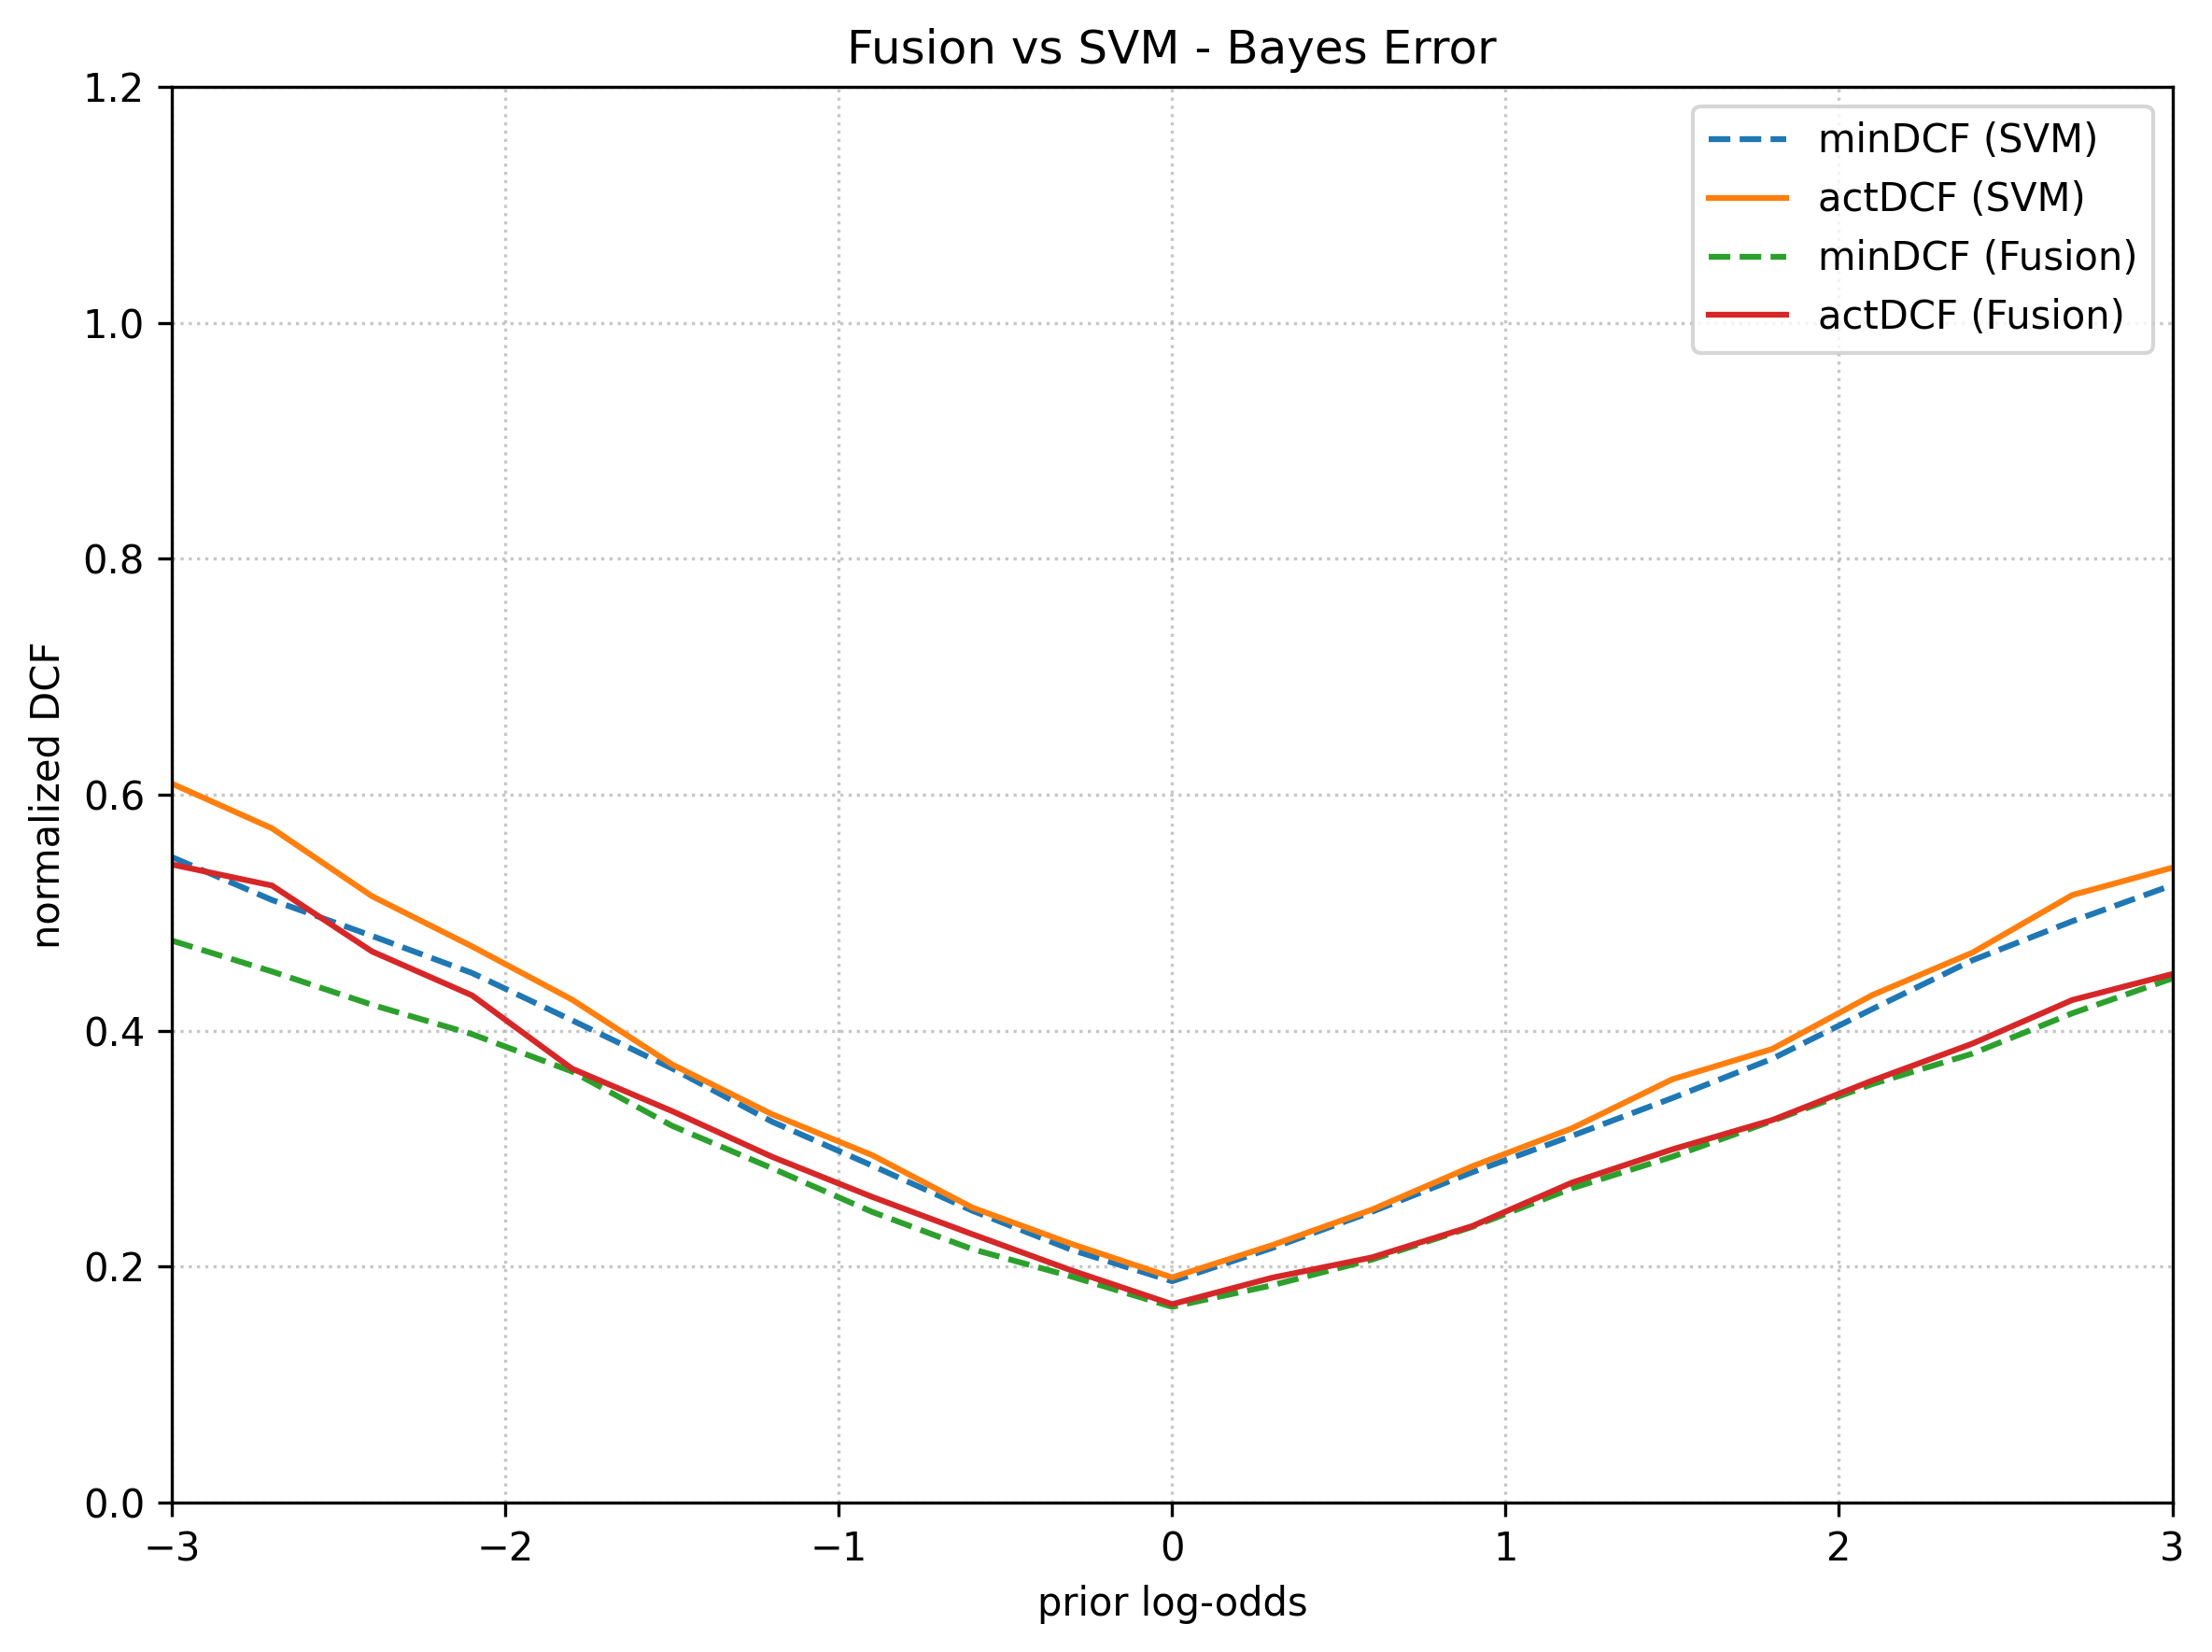
\includegraphics[width=\linewidth]{Bayes_Error_Fusion_vs_SVM.png}
\caption{Bayes Error: Fusion vs. Calibrated SVM.}
\label{fig:fusion_vs_svm}
\end{minipage}\hfill
\begin{minipage}{0.48\textwidth}
\centering
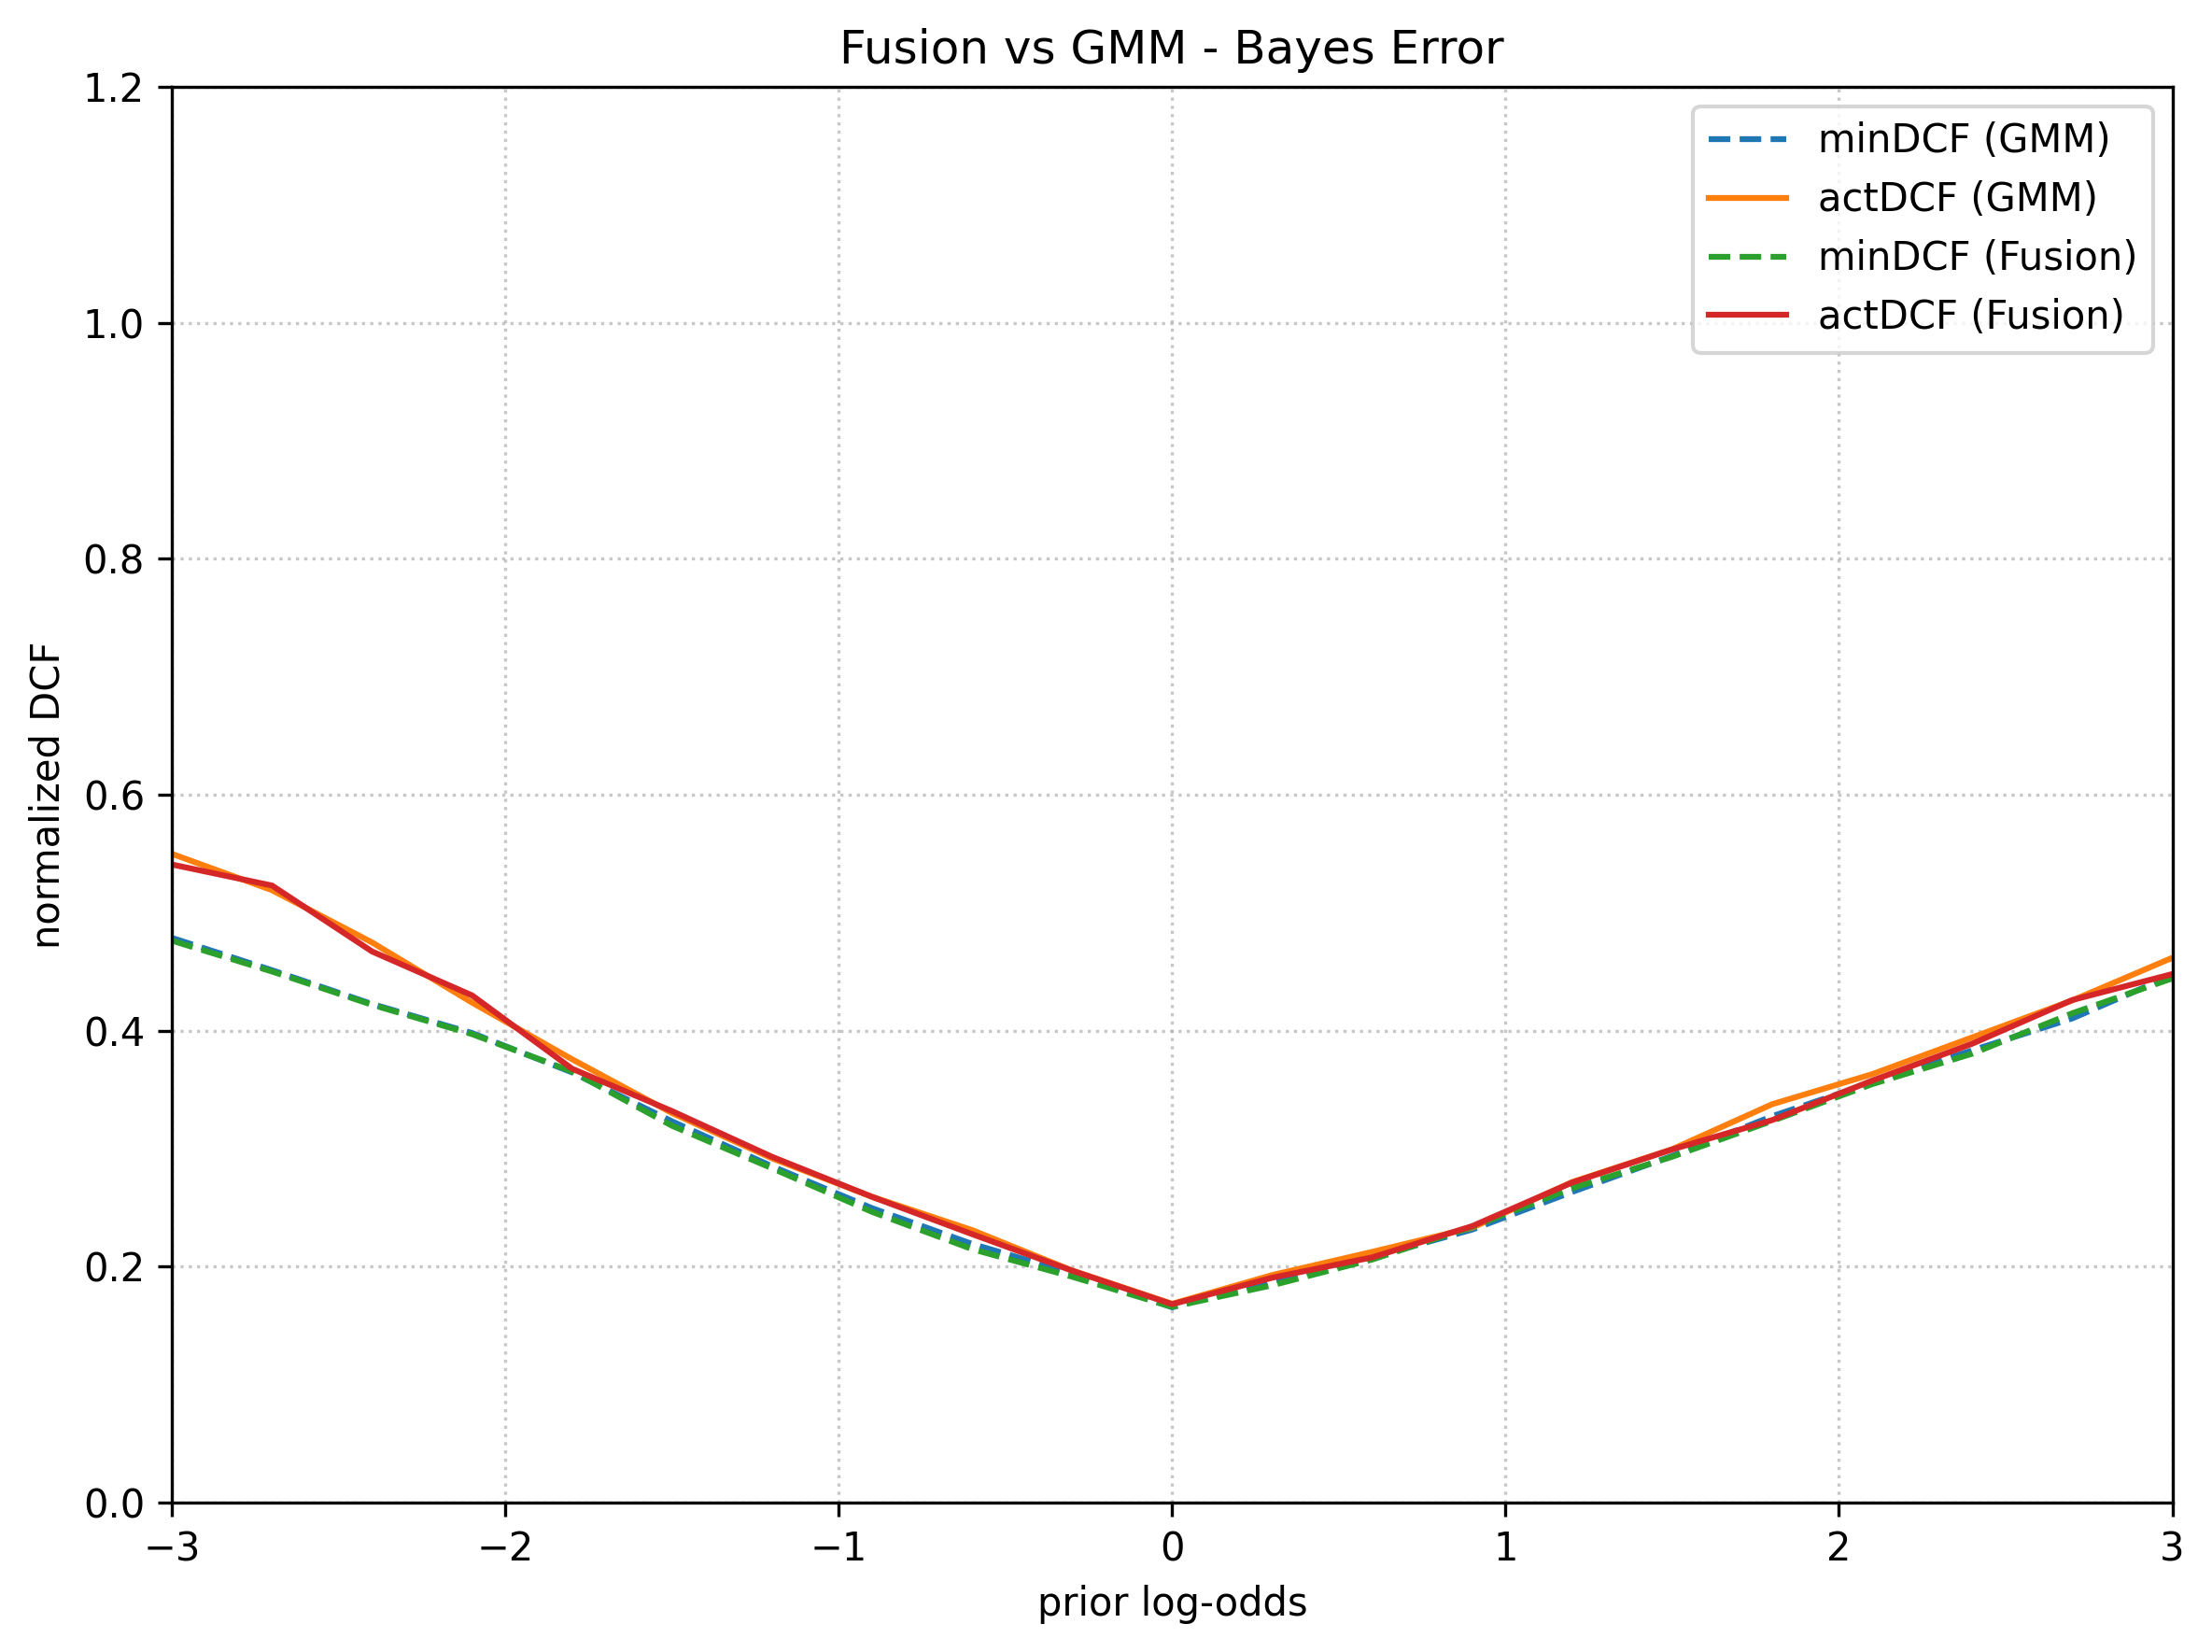
\includegraphics[width=\linewidth]{Bayes_Error_Fusion_vs_GMM.png}
\caption{Bayes Error: Fusion vs. Calibrated GMM.}
\label{fig:fusion_vs_gmm}
\end{minipage}
\end{figure}
\subsection*{Question: What do you observe when comparing the actual DCF error plots?}
Observing the comparative Bayes Error plots, the fused model's Actual DCF curve (red) consistently traces below or perfectly tracks the best available individual curve across the entire log-odds spectrum.
When compared to the SVM (Figure \ref{fig:fusion_vs_svm}), the fusion provides a massive, unmistakable reduction in both Actual and Minimum DCF at all operational points. When compared to the GMM (Figure \ref{fig:fusion_vs_gmm}), the improvement is much narrower, as the GMM is already highly performant. However, the fusion curve still manages to "shave off" the peaks of the GMM's Actual DCF at extreme log-odds, resulting in a system that is slightly more robust and better calibrated than the GMM alone.
\subsection*{Question: Was your final model choice effective?}
Yes, the final model choice (fusing the RBF SVM and the Tied GMM) was highly effective. At every evaluated prior ($\tilde{\pi}=0.1, 0.5, 0.9$), the fused system achieved a lower Minimum DCF than any individual model. For instance, at $\tilde{\pi}=0.9$, the fused system reached a Minimum DCF of \textbf{0.363} (compared to the GMM's 0.365 and SVM's 0.432) and maintained excellent calibration with an Actual DCF of \textbf{0.368}. This mathematically proves that the fusion successfully extracted complementary information from both models.
\subsection*{Question: Would another model/fusion of models have been more effective?}
It is highly unlikely that another combination within our tested architectures would have been more effective. While we could have included Quadratic Logistic Regression in the fusion stack, the results from Chapter 1 demonstrated that it was fundamentally outclassed by both the SVM and GMM in every scenario. Fusing a strictly inferior model (Quadratic LR), which suffers from heavy $L_2$-induced calibration distortion, with highly non-linear and better-calibrated models (RBF SVM, GMM) typically introduces more estimation noise than discriminative value. The pairing of SVM and GMM represents the optimal fusion strategy because they provide the maximum amount of geometric diversity.
\section{Theoretical Considerations}
The success of this Score-Level Fusion is deeply rooted in the concept of \textit{complementary error spaces}. For fusion to be mathematically advantageous, the constituent classifiers must make errors on different regions of the data distribution. Fusing models that fail on the exact same samples yields no improvement.
The RBF SVM and the Tied GMM provide this necessary diversity because they view the feature space through fundamentally opposed mathematical lenses:
\begin{itemize}
\item The \textbf{Tied GMM} is a \textit{generative} model. It assumes the data is generated by a mixture of localized Gaussian clusters and attempts to map the global probability density contours of the entire feature space.
\item The \textbf{RBF Kernel SVM} is a \textit{discriminative} model. It projects data into an infinite-dimensional space to find a strictly local, margin-maximizing boundary. It completely ignores the global density and focuses exclusively on the hardest-to-classify samples (the support vectors) near the boundary edge.
\end{itemize}
Because they utilize completely different geometric assumptions, their "blind spots" rarely overlap. As we observed in Laboratory 4, Features 5 and 6 exhibit heavy skewness with non-Gaussian drop-offs. The GMM, attempting to fit symmetric bells to these skewed tails, will naturally misclassify points lying in the distorted regions of the distribution. Conversely, the SVM makes no Gaussian assumptions; its local RBF kernel can perfectly wrap around those skewed drop-offs, correctly classifying the points the GMM missed.
The fusion Logistic Regression algorithm acts as a linear arbitrator. It learns an optimal plane in the 2D ($s_{\text{SVM}}, s_{\text{GMM}}$) score space, effectively discovering which model to trust in different regions of certainty. By linearly combining these diverse perspectives, the fused boundary becomes a highly robust meta-boundary, mitigating the individual architectural weaknesses of its components and achieving the lowest theoretical error rate on the evaluation set.